%%% Local Variables:
%%% mode: LaTeX
%%% TeX-master: "main"
%%% End:

\section{Общетехническое обоснование разработки устройства}

\subsection{Анализ исходных данных}

Рассматриваемым для проектированием устройстовом является сервотестер.
Устройство представляет собой печатную плату, с установленными на ней
навесным монтажом компонентами.

Данный тестовый стенд может работать в двух режимах, выбираемых переключателем:
\begin{enumerate} 
  
\item Ручной режим. В нём тестовый стенд генерирует импульсы для
четырех сервоприводов или полетного контроллера. Длина импульсов
контролируется четырьмя потенциометрами. В этом режиме тестовый стенд
обеспечивает питание сервоприводов или полетного контроллера и питание
от квадрокоптера не должно быть подключено к ним. Напряжение питания
тестового стенда должно быть между 7,5 или 12 Вольт.
  
\item Режим ввода. В нём измеряются длины имульсов поступающих от
приёмника сигнала. Сигналы потом поступают на выводы, подключенные к
полётному контроллеру или сервпоприводам.  В этом режиме тестовый
стенд и сервоприводы получают питание от источника питания от
квадрокоптера. Получаемое питание не должно превышать 7.49 Вольт и
тестовый стенд не должен быть подключен к своему истчонику
питания. Также четыре канада должны быть подключены, иначе светодиод и
зуммер просигналируют об ошибке.

\end{enumerate}

Сервотестер измеряет длину контрольных импульсов и даёт информацию о
качестве источника питания.


Информацию о сигналах выводимых к сервоприводам тестовый стенд выводит
на \textit{OLED} дисплей подключенный, через \textit{I2C} интерфейс.
Дисплей показывает продолжительсность импульсов графиком из четырёх
кривых вмести с их численным значением в микросекундах
~\cite{Elector521}.

Данное устройство может быть подключено между приёмником
дистанционного управления и полетным контроллером дрона, или между
полетным контроллером и сервоприводами.

\subsection{Формирование основных технических требований \\
  к разрабатываемой конструкции}

Так как в данном случае тестовый стенд используется для того, чтобы
тестировать отдельные компоненты и их взаимодействие, то логично
предположить, что в течении всего жизненного цикла изделия, оно не
будет покидать пределов лаборатории, в которой будут проводиться
испытания, осуществляемые на данном тестовом стенде.  Основываясь на
этом, можно говорить, что климатические условия эксплуатации данного
устройства соответствуют категории УХЛ 4.2 ГОСТ 15150-69.

Характеристика данной категории следующая:\\
Для эксплуатации в помещениях (объемах) с искусственно регулируемыми климатическими
условиями, например в закрытых отапливаемых или охлаждаемых и
вентилируемых производственных и других, в том числе хорошо
вентилируемых подземных помещениях (отсутствие воздействия прямого
солнечного излучения, атмосферных осадков, ветра, песка и пыли
наружного воздуха; отсутствие или существенное уменьшение воздействия
рассеянного солнечного излучения и конденсации влаги). Для эксплуатации
в лабораторных, капитальных и других подобного типа помещениях
~\cite{GOST-15150-69}.


\subsection{Схемотехнический анализ проектируемого средства}

Поскольку статья о тестовом сервотестере написана в иностранном журнале,
схема электрическая принципиальная в нём выполнена не по
отечественному ГОСТ.


\begin{figure}[h]
  \centering
  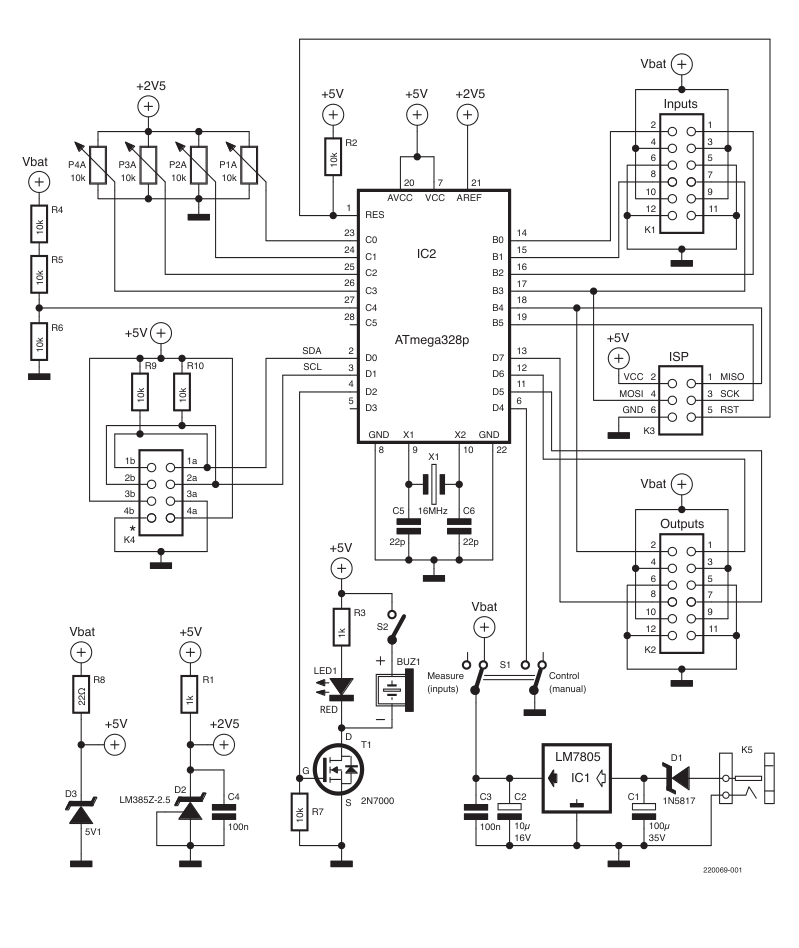
\includegraphics[scale = 0.60]{SchematicsShotFromElector.png}
  \caption{Электрическая принципиальная схема устройства}
\end{figure}

На приложенной схеме в центре видно микроконтроллер подключенный к
кристаллу с частотой колебаний 16 Мгц, который в свою очередь
подключен к конденсаторам C5 и С6. Четыре пина \textit{GPIO} — PB0-PB3
подключены к разъёму K1. Выводы для серво сигнала — PD5, PD6, PD7 и
PB4 подключены к разъёму K2. Два этих разъёма разведены таким
образом, что к ним можно подключить стандартный для сервопривода
кабель ~\cite{Elector521}.

Четыре потенциометра подключены к аналоговым входам микроконтроллера
PC0-PC3. Питание подключается через делитель напряжения из резисторов
R4-R6 к аналоговому входу PC4. Отношение между суммой сопротивлений
R4, R5 и сопротивлением R6 должно быть 2 к 1 соответственно, но их
абсолютные значения не критичны. Использование трёх резисторов одного
значения облегчает их сортировку для точности ~\cite{Elector521}.

Для того чтобы измерять напряжение источника питания нужен аналогово
цифровой преобразователь и опорное напряжение не относящиеся к самому
напряжению питания.  В микроконтроллере уже есть опорное напряжение в
1,1 Вольт, однако это значение несколько мало. И поэтому используется
источник опорного напряжения LM385-2.5 обозначенный как D2, как
внешнее опорное напряжение в 2,5 Вольта. Этот элемент более точен, чем
простой двух контактный зенеровский диод ~\cite{Elector521}.

К коннектору K4 подключается \textit{OLED} дисплей по типу SSD1306.  У
дисплея должен быть порт \textit{I2C}, но он будет подключаться к
порту \textit{I2C} микроконтроллера, но к компонентам PD0 и PD1. Шина
\textit{I2C} эмулируется программным обеспечением. Так выходит из-за
того, что шина \textit{I2C} на данном микроконтроллере находится на
том же пине, что и аналоговый вход PC4, который уже используется для
измерения напряжения питания ~\cite{Elector521}.

Резисторы R9 и R10 это подтягивающие резисторы для шины \textit{I2C}.

Ползунковый переключатель S1 типа \textit{DPDT} используется для
выбора режима работы сервотестера. В ручном режиме переключатель
соединяет напряжения питания номиналом 5 Вольт и коннекторы
сервоприводов. В режиме ввода он предотвращает неправильное включение
напряжений ~\cite{Elector521}.

Возможно, что решение в части подключение дисплея к данному тестовому
стенду и не является самым элегантным. Однако сама по себе схема
достаточно проста,состоит из небольшого числа компонентов, но тем не
менее может работать в нескольких режимах и схемах включения, что
выглядит как положительные черты относительно того в каких вариантах
использования оказывается устройство.
